\documentclass[13.5pt]{beamer}
\usepackage[natbib=true,backend=bibtex,useprefix=true]{biblatex}
\usepackage[utf8]{inputenc}
\usepackage{tikz}
\usepackage{ragged2e}
\usepackage{adjustbox}
\usepackage{amsmath}
\usepackage{amsfonts}
\usepackage{amssymb}
\usepackage{amsthm}
\usetikzlibrary{fadings}
\usepackage{fontspec}
\usepackage{unicode-math}
\setmathfont{XITS Math}


\usetheme{Madrid}

\definecolor{TorVergataColor}{RGB}{0,125,52}
\setsansfont[BoldFont={Circe-Bold}]{Circe-Regular}

\newcommand{\B}[1]{\textcolor{TorVergataColor}{\textbf{#1}}}
\newcommand{\Cross}{\mathbin{\tikz [x=2.5ex,y=2.5ex,line width=.10ex] \draw (0,0) -- (1,1) (0,1) -- (1,0);}}
\newcommand{\mathDef}{\overset{\textit{def}}{=}}
\newcommand{\N}{\mathbb{N}}
\newcommand{\R}{\mathbb{R}}
\newcommand{\Rplus}{\mathbb{R}^+}

\makeatletter
\setbeamertemplate{title page}{%
	\vbox{}
	\vfill
	{\usebeamercolor[fg]{titlegraphic}\inserttitlegraphic\par}
	\begingroup
	\centering
	\begin{beamercolorbox}[sep=8pt,center]{title}
		\usebeamerfont{title}\inserttitle\par%
		\ifx\insertsubtitle\@empty%
		\else%
		\vskip0.25em%
		{\usebeamerfont{subtitle}\usebeamercolor[fg]{subtitle}\insertsubtitle\par}%
		\fi%     
	\end{beamercolorbox}%
	\vskip1em\par
	\vfill%<- added
	\begin{beamercolorbox}[sep=8pt,left]{author}
		\usebeamerfont{author}\insertauthor
	\end{beamercolorbox}
	\vfill%<- added
	\begin{beamercolorbox}[sep=8pt,center]{institute}
		\usebeamerfont{institute}\insertinstitute
	\end{beamercolorbox}
	\vfill%<- added
	\begin{beamercolorbox}[sep=8pt,center]{date}
		\usebeamerfont{date}\insertdate
	\end{beamercolorbox}%
	\vskip0cm%<- changed
	%    
	\endgroup
	\vfill%<- removed
}
\makeatother



\setbeamercolor{structure}{fg=TorVergataColor}
\setbeamerfont{structure}{family=\bfseries,size=\large}

\title[]
{ 
	\textbf{A QoS-Aware Broker \\ for Multi-Provider Serverless Applications}
}

\author[Andrea Graziani (m. 0273395)]{{\Large \textbf{Andrea Graziani}}\\m. $0273395$\\[10mm]{\small 
		\begin{tabular}{l|l}
			\textbf{Supervisor}: & \textit{Valeria Cardellini } \\ 
			\textbf{Tutor}: & \textit{Gabriele Russo Russo}  \\  
\end{tabular}}}

\titlegraphic{
\includegraphics[width=9.5cm,height=2.4cm]{../Images/UniLogo/LogoMacroarea.png}}

\setbeamertemplate{background}{%
	\begin{tikzpicture}[overlay,remember picture]
		\node[scope fading=west,anchor=north west] at ([shift={(2in,-1in)}]current page.north west) {
\includegraphics[width=9cm,height=9cm]{../Images/UniLogo/TorVergataWatermark.png}};
	\end{tikzpicture}
}

\justifying

\setbeamertemplate{frametitle}{%
	\nointerlineskip%
	\begin{beamercolorbox}[wd=\paperwidth,ht=4.0ex,dp=1ex]{frametitle}
		\hspace*{1ex}\insertframetitle%
	\end{beamercolorbox}%
}

\addtobeamertemplate{frametitle}{}{%
	\begin{tikzpicture}[remember picture,overlay]
		\node[anchor=north east,yshift=2pt] at (current page.north east) {
\includegraphics[height=1cm]{../Images/UniLogo/NegativeTorVergataLogo.png}};
\end{tikzpicture}}

\date{May 23, 2022}

%-------------------------------------------------------
% THE BODY OF THE PRESENTATION
%-------------------------------------------------------

\begin{document}

%-------------------------------------------------------
% THE TITLEPAGE
%-------------------------------------------------------

{% % this is the name of the PDF file for the background
\begin{frame}[plain,noframenumbering] % the plain option removes the header from the title page, noframenumbering removes the numbering of this frame only
  \titlepage % call the title page information from above
\end{frame}}

\setbeamertemplate{background}{}

% -------------- %
% -------------- %
\begin{frame}{Goals}
% -------------- %
% -------------- %

\begin{block}{}
	\centering
	My thesis is focused on ``\B{Serverless Computing}".
\end{block}

\vspace{\baselineskip}
Two main goals:
\begin{enumerate}
	\item The \B{orchestration} of a serverless workflow supporting:
	
	\begin{itemize}
		\item \textbf{Multiple FaaS Providers}
		\item \textbf{Multiple Functions Implementations.}
	\end{itemize}
	\vspace{\baselineskip}
	\item The fulfillment of \B{non-functional requirements} concerning the \B{quality of service} (QoS) levels that should be guaranteed.
\end{enumerate}

\end{frame}
% -------------- %
% -------------- %
\begin{frame}{Serverless Computing: Overview}


\begin{block}{}
\centering
What's meant by serverless computing?
\end{block}
\vspace{\baselineskip}
An applications service model where:
\vspace{\baselineskip}
\begin{itemize}
	\item Administration tasks (provisioning, monitoring, scaling, etc.) are directly managed by the provider.
	\vspace{\baselineskip}
	\item Small-granularity billing pricing model: \B{pay-as-you-go}.
	\vspace{\baselineskip}
	\item Cloud application are abstracted as a group of so-called \\ ``\B{Serverless Functions}".
	
\end{itemize}

\end{frame} 
% -------------- %
% -------------- %
\begin{frame}{Serverless Computing: Overview}
	
	\begin{block}{}
		\centering
		What is a serverless function?
	\end{block}
	\vspace{\baselineskip}
	A computation unit implementing a business functionality.
	
	\begin{itemize}
		\item \B{Stateless}
		\item \B{Event-Driven}
		\item \B{Short-Lived}
	\end{itemize}

\end{frame} 
% -------------- %
% -------------- %
\begin{frame}{Serverless Computing: Overview}
	
	\begin{block}{}
		\centering
		A serverless function is executed inside a containerized environment: the so-called ``\B{Function Instance}".
	\end{block}
	\vspace{\baselineskip}
	Any function instance can be in:
	\begin{itemize}
		\item Initialization State.
		\item Idle State.
		\item Running State
	\end{itemize}
	\vspace{\baselineskip}
	\begin{block}{\textbf{Warm Pool}}
		
		The set of all function instances whose state is either \B{idle} or \B{running} state.
	\end{block}
	
	
	
\end{frame} 
% -------------- %
% -------------- %
\begin{frame}{Serverless Computing: Overview}
	
\begin{block}{}
	\centering
	The FaaS platform \B{automatically} scales the number of function instances.
\end{block}

\vspace{\baselineskip}
When a request comes in, only one of the following events can occur:
\begin{itemize}
	\item \textbf{Warm start}.
	\item \textbf{Cold start.}
\end{itemize}

		
\end{frame} 
% -------------- %
% -------------- %
\begin{frame}{Serverless Computing: Overview}
	
	\begin{block}{Concurrency Level}
		The limitation, imposed by FaaS platforms, on the \B{number} of function instance runnable at the \B{same time}.
	\end{block}
	\vspace{\baselineskip}
	Providers apply that restriction differently:
	\vspace{\baselineskip}
	\begin{itemize}
		\item \B{Global (Per-Account) Concurrency Model}.
		\begin{itemize}
			\item AWS Lambda. 
			\item IBM Cloud Functions.
		\end{itemize}
		\vspace{\baselineskip}
		\item \B{Local (Per-Function) Concurrency Model}.
		\begin{itemize}
			\item Google Cloud Functions.
		\end{itemize}
	\end{itemize}

\end{frame} 
% -------------- %
% -------------- %
\begin{frame}{Serverless Computing: Problems}
	
	\begin{block}{}
		\centering
		What current problems or limitations of the serverless computing paradigm I tried to solve?
	\end{block}
\vspace{\baselineskip}
	\begin{itemize}
		\item Vendor lock-in issues.
		\item The fulfillment of quality of service (\textit{QoS}) levels.
	\end{itemize}

\end{frame} 
% -------------- %
% -------------- %
\begin{frame}{Serverless Computing: Problems}
	
	\begin{block}{}
		\centering
		Why is so difficult to guarantee QoS levels?
	\end{block}
	\vspace{\baselineskip}
	\begin{itemize}
		\item Lack of an analytical model to predict application performance.
		\vspace{\baselineskip}
		\item Lack of a methodological way to find a suitable ``\B{configuration}" for a serverless application.
	\end{itemize}

\end{frame} 
% -------------- %
% -------------- %
\begin{frame}{Serverless Computing: Problems}
	
	\begin{block}{}
		\centering
		Why is so difficult to find a suitable configuration for a \\serverless application?
	\end{block}
	\vspace{\baselineskip}
	Configuration parameters \textbf{significantly} affect the \textbf{cost} and \textbf{response time} of serverless functions.
	
	\begin{figure}[h]
		\centering
		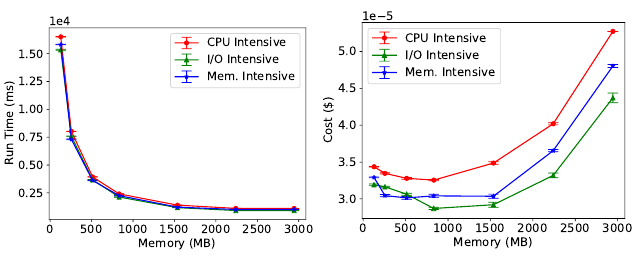
\includegraphics[width=\textwidth]{../Images/slideImage1.png}
	\end{figure}
	
\end{frame} 
% -------------- %
% -------------- %
\begin{frame}{Related Works}

Solutions \textbf{already} exist, \textbf{but}:
\vspace{\baselineskip}
\begin{itemize}
	\item They are unaware of the current status of FaaS platforms.
	\item No support for multiple implementations, or versions, of a same serverless function.
	\item No support for multiple FaaS platforms.
	\item Limited support for generic workload applications.
\end{itemize}

\end{frame} 

% -------------- %
% -------------- %

\begin{frame}{My Contributions}
	
	My contributions respect to the current state of art:
	\vspace{\baselineskip}
	\begin{enumerate}
	
		\item An \B{Analytical Model} to evaluate applications performance.
		\begin{itemize}
			\item Multi-Provider.
			\item Multi-Implementation.
			\item QoS-Aware.
			\item FaaS-Status-Aware.
		\end{itemize}
		\vspace{\baselineskip} 
		\item A \B{methodological way} to find the ``best" configuration to satisfy QoS constraints.
		\begin{itemize}
			\item By solving an optimization problem.
		\end{itemize}
		\vspace{\baselineskip} 
		
	\end{enumerate}
	
\end{frame} 

% -------------- %
% -------------- %

\begin{frame}{My Contributions}
	
	\vspace{\baselineskip}
	\begin{enumerate}
		\justifying
		\setcounter{enumi}{2}
		\item A custom \B{heuristic algorithm} to resolve the aforementioned optimization problem.
		\vspace{\baselineskip} 
		\item A \B{software framework} for the orchestration of serverless applications supporting ``hybrid-scheduling".
		\begin{itemize}
			\item Following REST architectural style.
		\end{itemize}
		\vspace{\baselineskip} 
		\item An extension to an already existent \B{representation scheme} to define a serverless application workflow.
		\vspace{\baselineskip} 
		
		
	\end{enumerate}
	
\end{frame} 

% -------------- %
% -------------- %

\begin{frame}{The Software Framework}
	
 	Main features of our software framework:
	\vspace{\baselineskip}
	\begin{itemize}
		\item \B{Client-Server architecture}.
		\item \B{Cloud-native} application.
		\item Includes a set of \B{adapters} to interact with following FaaS providers:
		\begin{itemize}
			\item AWS Lambda.
			\item Apache OpenWhisk.
		\end{itemize}
		\item \B{REST} architectural style.
	\end{itemize}
	
\end{frame} 
% -------------- %
% -------------- %
\begin{frame}{The Software Framework}
	
	Main logical entities of our system:
	
	\begin{itemize}
		\item A Logging subsystem.
		\item An Orchestrator.
		\item A profiler.
		\item A QoS-aware model-based optimizer.
		\item A Custom AFCL Parser.
	\end{itemize}
	
\end{frame} 

% -------------- %
% -------------- %
\begin{frame}

\begin{figure}[h]
	\centering
	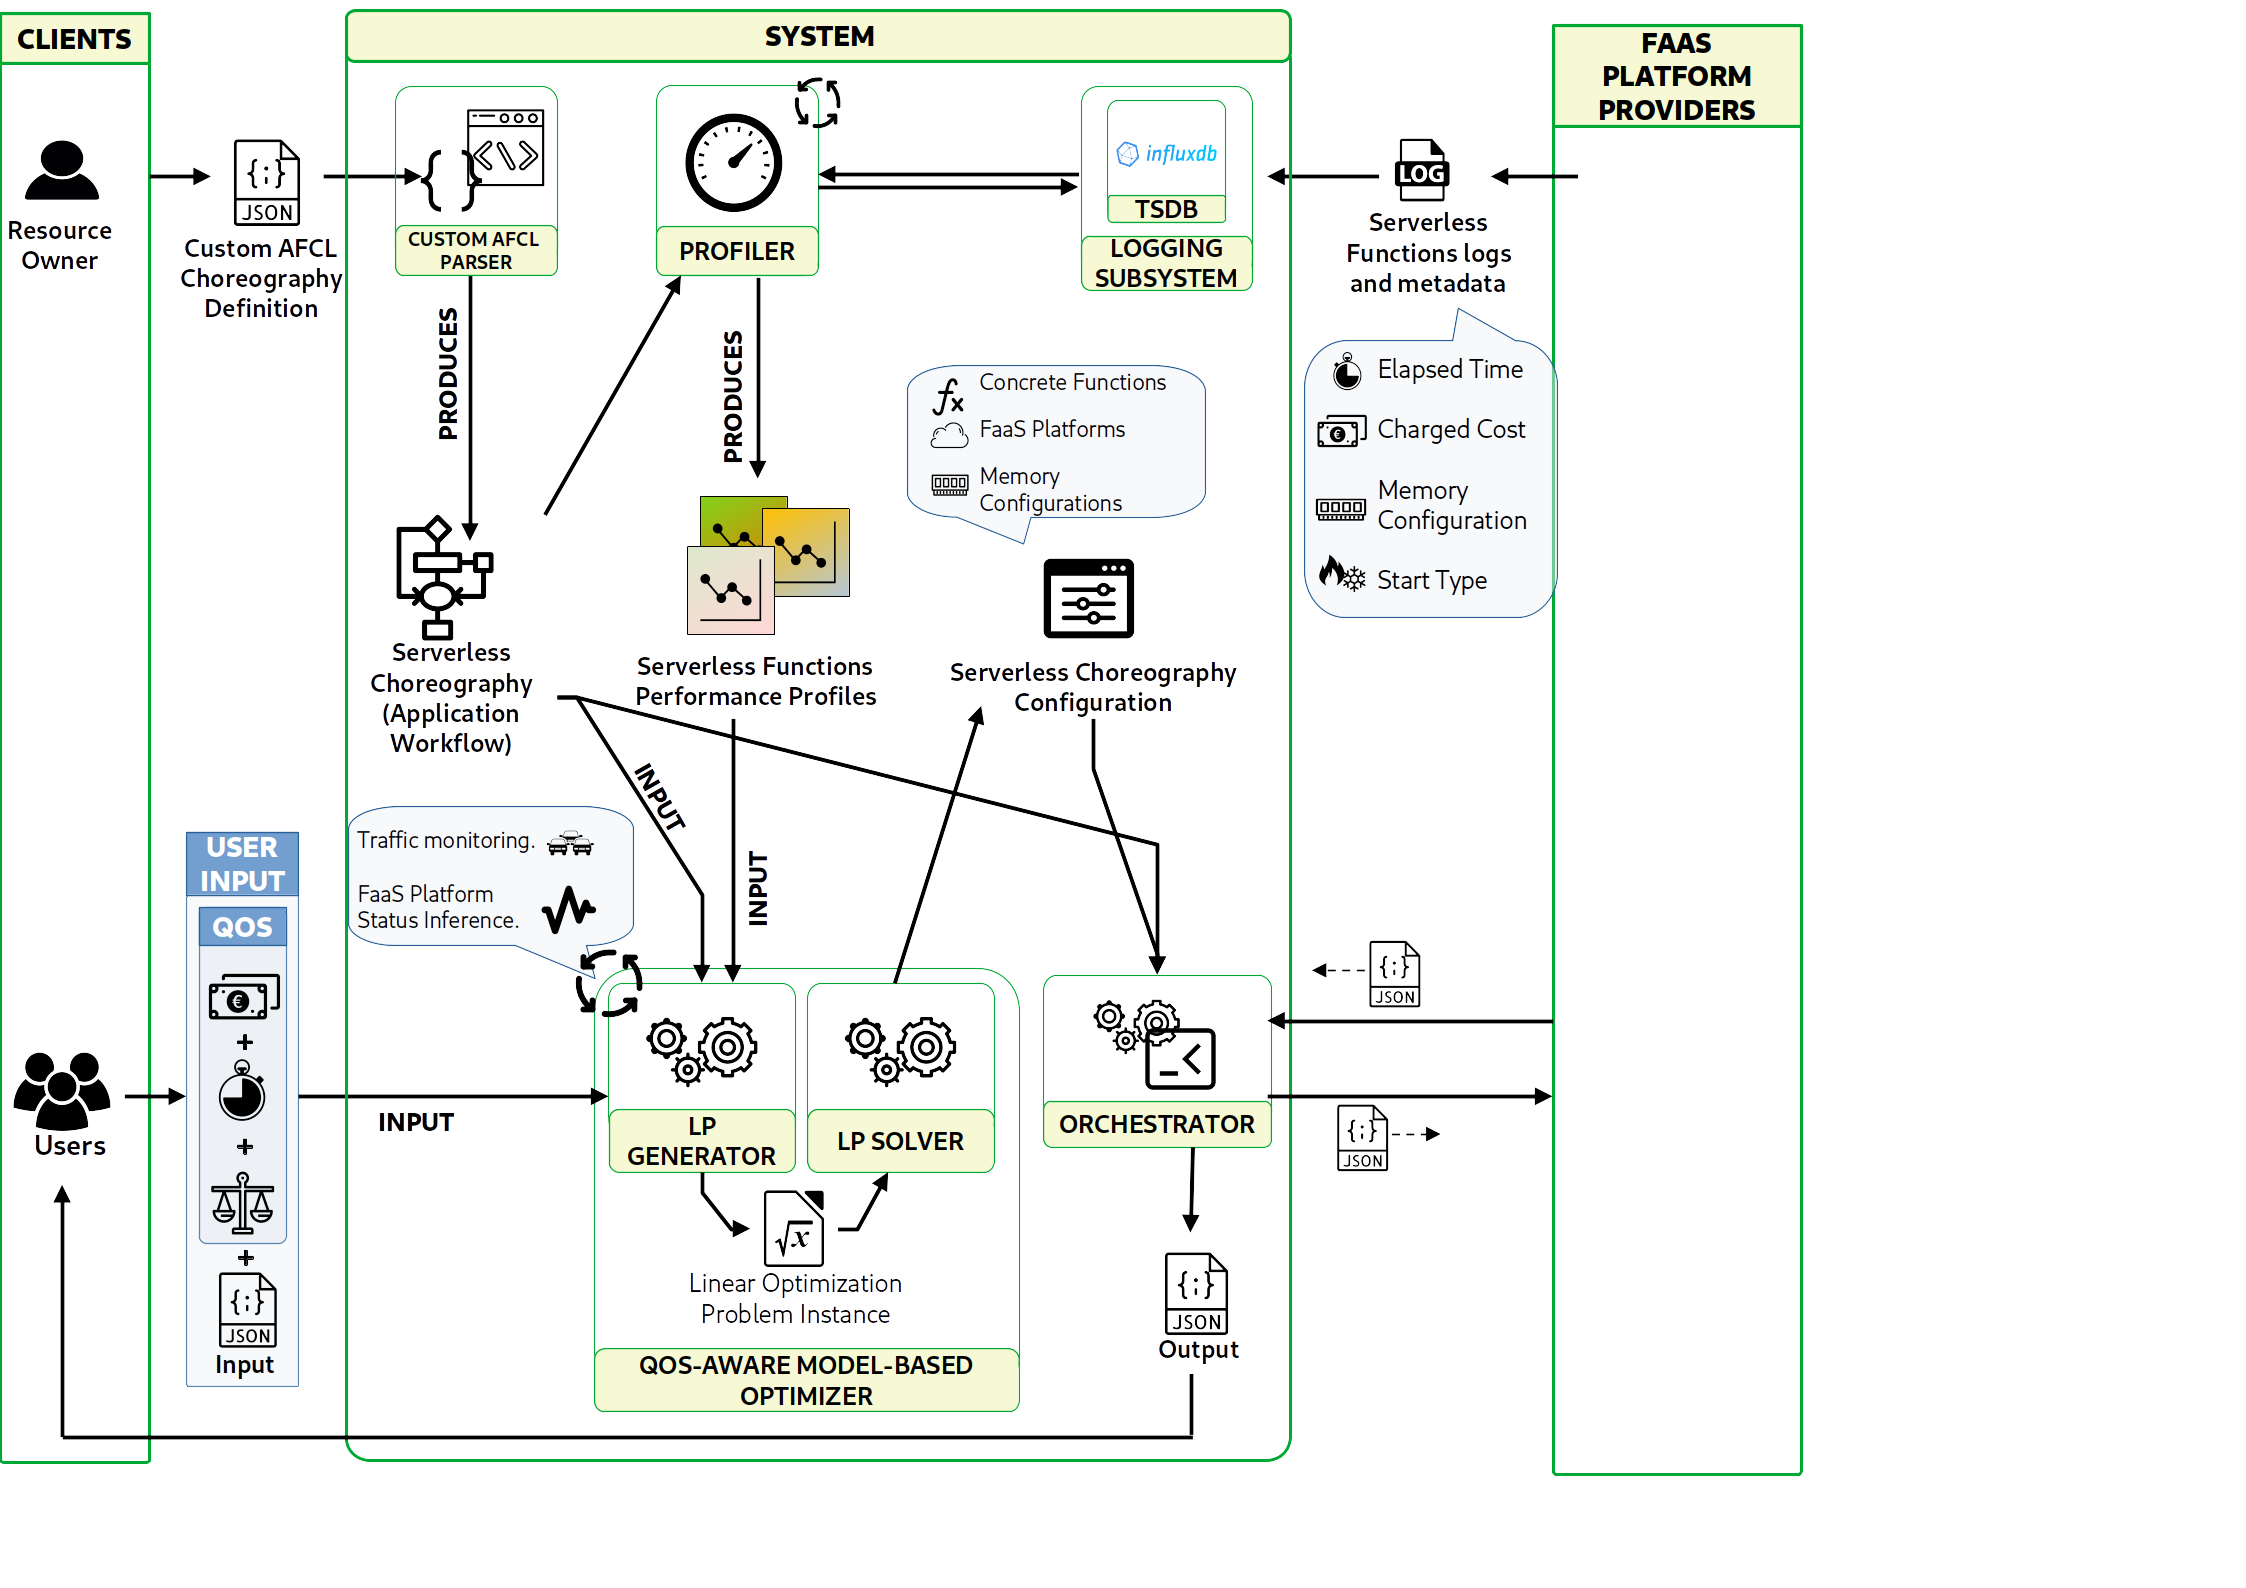
\includegraphics[width=\textwidth]{../Images/SystemForSlide.png}
\end{figure}


\end{frame} 
% -------------- %
% -------------- %
\begin{frame}{The Software Framework}
	
	\begin{block}{}
		\centering
		An unique representation scheme is used for serverless workflows.
	\end{block}

	\vspace{\baselineskip}
	
	\begin{itemize}
		\item It is based on an existing language called \B{Abstract Function Choreography Language} (AFCL).
		\item I extend the original one to include the support for multiple serverless function implementations hosted on multiple FaaS.
	\end{itemize}

	\vspace{\baselineskip}
	
	\begin{block}{Advantages}
	\centering
	\begin{itemize}
		\item Access transparency.
		\item It overcomes portability limitations and vendor lock-in issues.
	\end{itemize}
	\end{block}
	

\end{frame} 
% -------------- %
% -------------- %
\begin{frame}{The Analytical Model}
	
	
	
	
	Informally, that abstraction has been derived from that of a \textit{control-flow graph} which, as known, describes, using graphs notation, all paths that might be traversed through a serverless application during its execution. Similarly, a choreography describes calling relationships between functions belonging to an application in a serverless environment, combining them using several types of control-flow structures, like sequence, branch, loop or connectors for a parallel execution. 
	

	
\end{frame} 
% -------------- %
% -------------- %
\begin{frame}{System Model}
	
	
	
\end{frame} 
% -------------- %
% -------------- %
\begin{frame}{System Model}
	
Formally, let a choreography $\mathcal{C} = (\Phi,E)$, when an invocation request of $\mathcal{C}$ arrive on our system, the latter acts as follows:

\begin{itemize}
	\item For each $\phi \in \mathcal{F_E}(\mathcal{C})$, it selects only one concrete function $f_{\phi} \in \textbf{F}_{\phi}$, which will be effectively invoked and executed on its corresponding FaaS platform. 
	\item For each selected concrete function $f_{\phi}$, it selects a value for memory size.
\end{itemize}
	
\end{frame} 
% -------------- %
% -------------- %
\begin{frame}{System Model}
	
According to our model point of view, at any time $t$, any FaaS platform provider acts as a ``\textit{set}'' of $M/G/K(t)_{\textbf{C}_{max}}/K(t)_{\textbf{C}_{max}}$ queueing systems, also called \textit{$K(t)$-server loss systems}, where:
	
\end{frame}


\begin{frame}
	Then, let $\phi \in \mathscr{F_E}(\mathcal{C})$ an executable function and $\textbf{F}_{\phi}$ the corresponding implementation-set, formally an \textit{executable function configuration} $x_{\phi}$ for the executable function $\phi$ is a two-dimensional vector defined as follows:
	
	\begin{equation}
		x_{\phi} = (f_{\phi},m) \in f_{\phi} \times \textbf{M}_{f_{\phi}} \subseteq \textbf{F}_{\phi} \times \N
	\end{equation}
	
	where:
	
	\begin{itemize}
		\item $f_{\phi} \in \textbf{F}_{\phi}$  denotes a particular concrete function implementing the executable function $\phi$.
		\item $m \in \textbf{M}_{f_{\phi}}$ represents the allocated memory size during the execution of $f_{\phi}$, where $\textbf{M}_{f_{\phi}} \subseteq \N$ is the set holding all available memory size configurations allowed by provider where the concrete function $f_{\phi}$ is executed.
	\end{itemize}
\end{frame}


\begin{frame}
	Formally, a \textit{serverless choreography configuration} $\textbf{X}_{\mathcal{C}}$ for the choreography $\mathcal{C}$ is a vector such that:
	
	\begin{eqnarray}
		\textbf{x}_{\mathcal{C}} & \mathDef & \left\lbrace x_{\phi_{1}}, \ldots, x_{\phi_{k}} \right\rbrace \nonumber \\ 
		& \in & \left\{  \left\{ \bigcup_{j=1}^{|\textbf{F}_{\phi_{1}}|} f_{\phi_{1_j}} \times \textbf{M}_{f_{\phi_{1_j}}} \right\} \times \ldots \times \left\{ \bigcup_{j=1}^{|\textbf{F}_{\phi_{k}}|} f_{\phi_{k_j}} \times \textbf{M}_{f_{\phi_{k_j}}} \right\} \right\}  \nonumber \\
		& = & \Cross_{i = 1}^k \left\{ \bigcup_{j=1}^{|\textbf{F}_{\phi_{i}}|} f_{\phi_{i_j}} \times \textbf{M}_{f_{\phi_{i_j}}} \right\} \nonumber \\
		& \subseteq & \Cross_{i = 1}^k \left\{ \textbf{F}_{\phi_{i}} \times \mathbb{N} \right\} = \textbf{X}_{\mathcal{C}}
	\end{eqnarray}

	\begin{block}{Concrete Functions}
		\centering
		Set of semantically and logically equivalent serverless function implementations, accepting the same set of input data and returning the same type of output data. They may expose different performance or cost behavior.
	\end{block}

\end{frame}


% -------------- %
% -------------- %

\setbeamertemplate{background}{%
	\begin{tikzpicture}[overlay,remember picture]
		\node[scope fading=west,anchor=north west] at ([shift={(2in,-1in)}]current page.north west) {
\includegraphics[width=9cm,height=9cm]{../Images/UniLogo/TorVergataWatermark.png}};
	\end{tikzpicture}
}

\begin{frame}{{}}
	\begin{block}{}
		\centering
		Thanks for your attention!\\\B{Questions}?
	\end{block}
\end{frame} 



\begin{frame}
	Formally, a \textit{serverless choreography configuration} $\textbf{X}_{\mathcal{C}}$ for the choreography $\mathcal{C}$ is a vector such that:
	
	\begin{eqnarray}
		\textbf{x}_{\mathcal{C}} & \mathDef & \left\lbrace x_{\phi_{1}}, \ldots, x_{\phi_{k}} \right\rbrace \nonumber \\ 
		& \in & \left\{  \left\{ \bigcup_{j=1}^{|\textbf{F}_{\phi_{1}}|} f_{\phi_{1_j}} \times \textbf{M}_{f_{\phi_{1_j}}} \right\} \times \ldots \times \left\{ \bigcup_{j=1}^{|\textbf{F}_{\phi_{k}}|} f_{\phi_{k_j}} \times \textbf{M}_{f_{\phi_{k_j}}} \right\} \right\}  \nonumber \\
		& = & \Cross_{i = 1}^k \left\{ \bigcup_{j=1}^{|\textbf{F}_{\phi_{i}}|} f_{\phi_{i_j}} \times \textbf{M}_{f_{\phi_{i_j}}} \right\} \nonumber \\
		& \subseteq & \Cross_{i = 1}^k \left\{ \textbf{F}_{\phi_{i}} \times \mathbb{N} \right\} = \textbf{X}_{\mathcal{C}}
	\end{eqnarray}
\end{frame}





\end{document}
